\begin{figure}[H]
	\begin{center}
		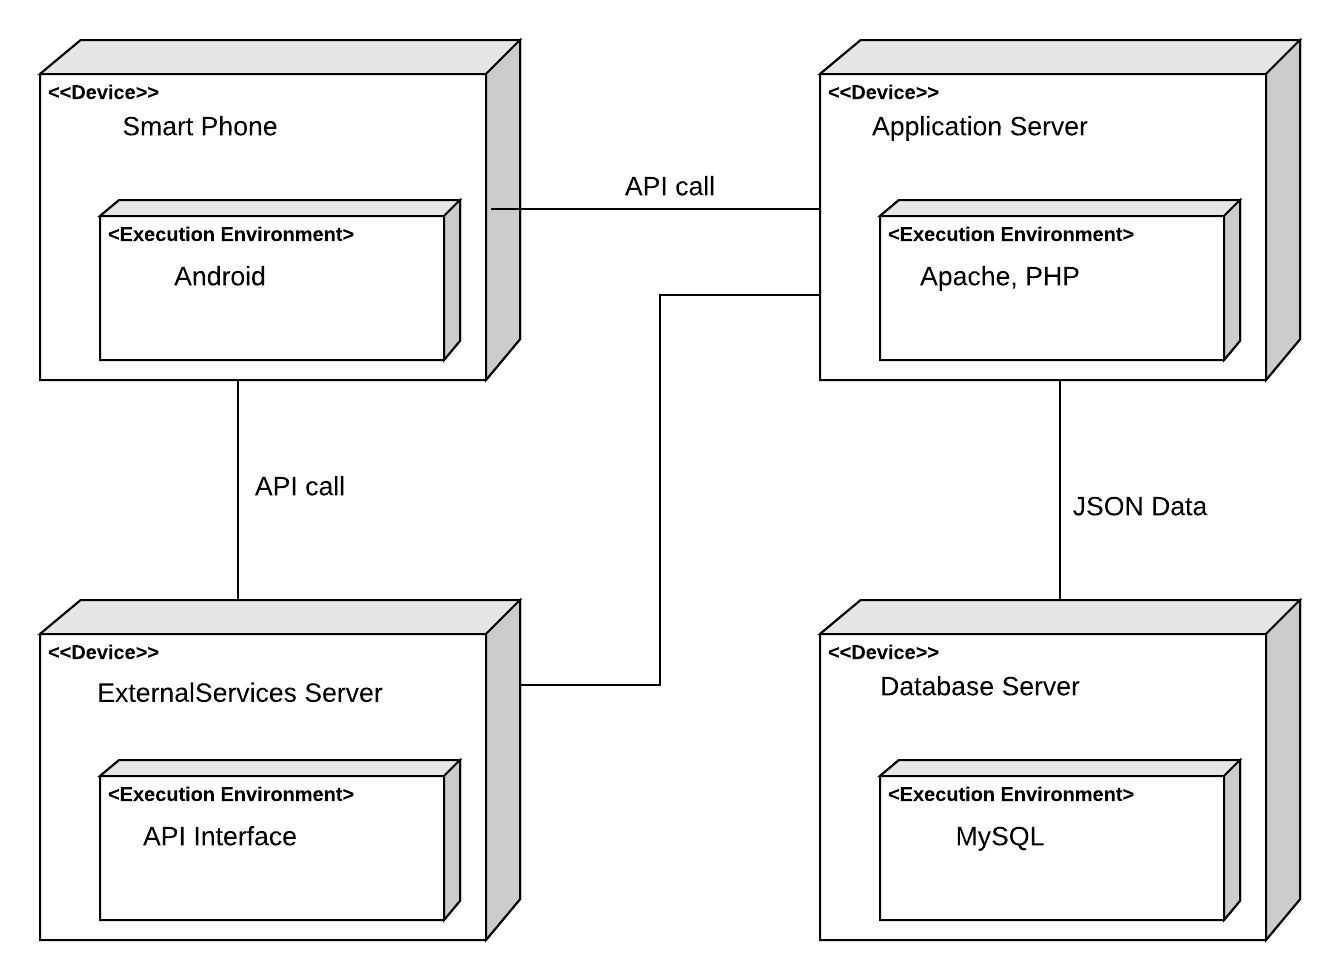
\includegraphics[width=\textwidth]{./DD_Diagrams/Deployment.png}
      \caption{Deployment Diagram}
        \label{TrackMe_depdia}
	\end{center}
\end{figure}
It shows architecture of the system as deployment (distribution) of software artifacts to deployment targets. Artifacts represent concrete elements in the physical world that are the result of a development process which are \textit{Android, Apache, PHP, API Interface} and \textit{MySQL}. Deployment target is usually represented by a node which is either hardware device or some software execution environment which are \textit{Smart Phone, Application Server, External Service Server} and \textit{Database Server}. The nodes are connected through communication paths to create networked systems of arbitrary complexity.\newline
The nodes an their respective artifacts are explained below:
\begin{itemize}
\item \textbf{Smart Phone:} The user uses smart phone to view the mobile application of the system. This is implemented in the execution environment Android which is artifact of this device.\newline
-\textit{Android:} The Android application can be built using any platform. It takes the information from external API's and the database server of the application to process and show information to the user using XML design techniques and Java Script codes.
\item \textbf{Application Server:} The Application Server is the host of the application and the database server. It is the central system of the entire application which manages the transfer and retrieval of data. The execution environment here is Apache and PHP.\newline
-\textit{Apache and PHP: } The Server does all the transaction on the database and manages the retrieval and transfer of data from and to database by using PHP code. We use PHP code to help convert the database into an API in JSON format which can be easily used by the application's front end to use the data.
\item \textbf{Database Server:} It stores all the data which is used by the application. The execution environment is MySQL.\newline
-\textit{MySQl:} MySQL database is used to store the details where the data can be easily stored from the form the user fills in the application. 
\item \textbf{ExternalServices Server:} It contains the information of all the external servers required by the application. The information from the server by using the API Interface.\newline
-\textit{API Interface:} The API provides the data in the JSON format which is fetched in the android platform by API call. 


\end{itemize}

